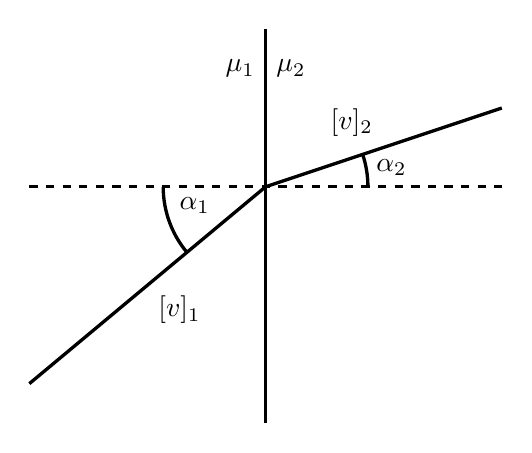
\begin{tikzpicture}[line width = 1.2pt, line join=round,x=1cm,y=1cm,>=stealth]
	% Grenzschicht
	\draw (0,-3) -- (0,2);
	% Referenznormale
	\draw [dashed] (-3,0) -- (3,0);
	% magnetischen Flussdichten
	\draw (-3,-2.5) -- (0,0);
	\draw ({-3/2},{-2.5/2}) node[anchor=north west] {$ \tetB[v]_1 $};
	\draw (0,0) -- (3,1);
	\draw ({3/2},{1/2}) node [anchor=south east] {$ \tetB[v]_2 $};
	% Winkel
	\draw (-1.3,0) arc (180:220:1.3);
	\draw (-0.9,0) node[anchor=north] {$ \alpha_1 $};
	\draw (1.3,0) arc (0:19:1.3);
	\draw (1.6,0) node[anchor=south] {$ \alpha_2 $};
	% Permeabilität
	\draw (0,1.5) node[anchor=east] {$ \mu_1 $};
	\draw (0,1.5) node[anchor=west] {$ \mu_2 $};
\end{tikzpicture}